\claude{
\Needspace{8\baselineskip}
\section[Dimension recovery and periodic motion]{Dimension recovery and periodic motion}\label{sec:controlled}
A diagonal matrix with oscillating entries provides an exact comparison. Its dimension is the number of independent oscillations, and MG tracks that number (\appref{app:controlled}). We then vary the loss weights of a digit classifier to induce oscillations in its trainable parameters. The loss weights set the frequencies, and covariance across training steps shows which weight directions vary.

For the classifier we compare MG with the participation ratio (PR) of the weight covariance. PR is $(\sum_i v_i)^2/\sum_i v_i^2$ for covariance eigenvalues $v_i$ and equals $r$ when $r$ directions have equal nonzero variance. We keep the estimator settings fixed across evaluation runs. Parameter logs and loss on fixed examples give more accurate estimates than gradient norm (Table~\ref{tab:synthetic-errors}).

\begin{table}[htbp]
\centering\small
\setlength{\tabcolsep}{2.5pt}
\caption{\cx{Digit classifier errors against weight covariance PR across held-out rank--repeat pairs.}}
\label{tab:synthetic-errors}
\begin{tabular}{lr}
\toprule
Recorded quantity & \cx{Mean absolute error} \\
\midrule
Parameter norm & \cx{0.57} \\
Loss on fixed examples & \cx{0.59} \\
Fixed parameter projection & \cx{0.62} \\
Gradient norm & \cx{1.70} \\
\bottomrule
\end{tabular}
\end{table}

In linear regression, a mode is an oscillating component of the weight error along a Hessian eigenvector. Damping selected modes lowers MG@loss while all weights remain trainable (Figure~\ref{fig:components}).

\subsection{Learned generators distinguish phases from harmonics}\label{sec:generator}
Several spectral peaks can arise from harmonics of one oscillation or from independent oscillations. We train recurrent networks to produce both kinds of signal using first-order reduced and controlled error (FORCE) learning \citep{sussillo2009generating}. FORCE adjusts the output weights to reproduce a prescribed signal and feeds each output back into the state. We then fix the weights and compute MG from one neuron's activation recorded at each simulated step. MG separates \cx{generators whose summed outputs have the same number of peaks and whose full-state covariance PRs are similar} (Figure~\ref{fig:components}). At higher dimension, MG overestimates the number of independent oscillations and the estimates overlap (Table~\ref{tab:generator_phases}).

\cx{The numeral in each task label counts output frequencies. In T2, the two frequencies have independent phases. In H2, one frequency is twice the other, so one phase determines both. M4 combines two independent frequencies and their second harmonics.}

\begin{figure*}[htbp]
\centering
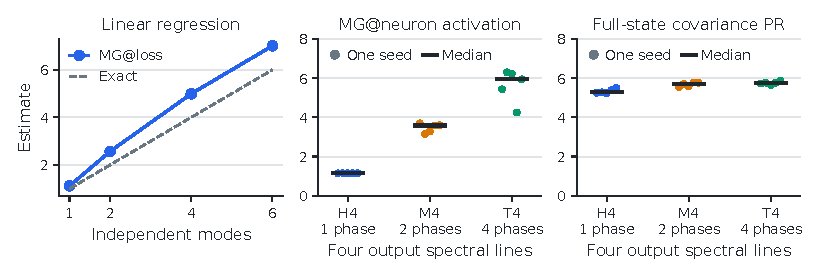
\includegraphics[width=.98\textwidth]{figures/components.pdf}
\caption{Left, MG@loss tracks how many independent oscillations (modes) contribute to the weight error in linear regression. Center and right, generators with four peaks \cx{in the summed output} and different numbers of independent phases. Dots show runs and bars show medians. MG separates phase counts more clearly than the covariance PR of activation vectors across all neurons.}
\label{fig:components}
\end{figure*}

\begin{table}[htbp]
\centering\small
\caption{Phase structure in learned generators. Entries show mean $\pm$ standard deviation across five runs. \cx{MG uses one neuron and PR uses all activations.}}
\label{tab:generator_phases}
\begin{tabular}{lrrr}
\toprule
Task & Phases & MG & Covariance PR \\
\midrule
T1 & 1 & \cx{$1.14 \pm 0.03$} & \cx{$1.66 \pm 0.08$} \\
T2 & 2 & \cx{$2.80 \pm 0.09$} & \cx{$2.98 \pm 0.07$} \\
T3 & 3 & \cx{$6.37 \pm 1.29$} & \cx{$4.36 \pm 0.10$} \\
T4 & 4 & \cx{$5.62 \pm 0.84$} & \cx{$5.75 \pm 0.08$} \\
H2 & 1 & \cx{$1.05 \pm 0.18$} & \cx{$2.94 \pm 0.09$} \\
H4 & 1 & \cx{$1.151 \pm 0.001$} & \cx{$5.33 \pm 0.11$} \\
M4 & 2 & \cx{$3.46 \pm 0.24$} & \cx{$5.67 \pm 0.11$} \\
\bottomrule
\end{tabular}

\end{table}

\subsection{FORCE training from chaos to periodic output}\label{sec:force}
We use FORCE to train networks with chaotic initial dynamics to reproduce a prescribed two-dimensional periodic signal. At selected training steps, we take the current state and simulate the network with the weights held fixed. Along this sequence of states, called a rollout, we record one neuron's activation. MG approaches one, the dimension of a closed periodic orbit (Figure~\ref{fig:force-log-geometry}).

We estimate finite-time Lyapunov exponents, the average exponential growth rates of small perturbations to the full hidden state. We select initial networks with a positive largest exponent. Most trained networks pass a test for stable periodic motion that checks the state return after one period and contraction in directions transverse to the orbit (Table~\ref{tab:force-outcome}).

\begin{figure*}[htbp]
\centering
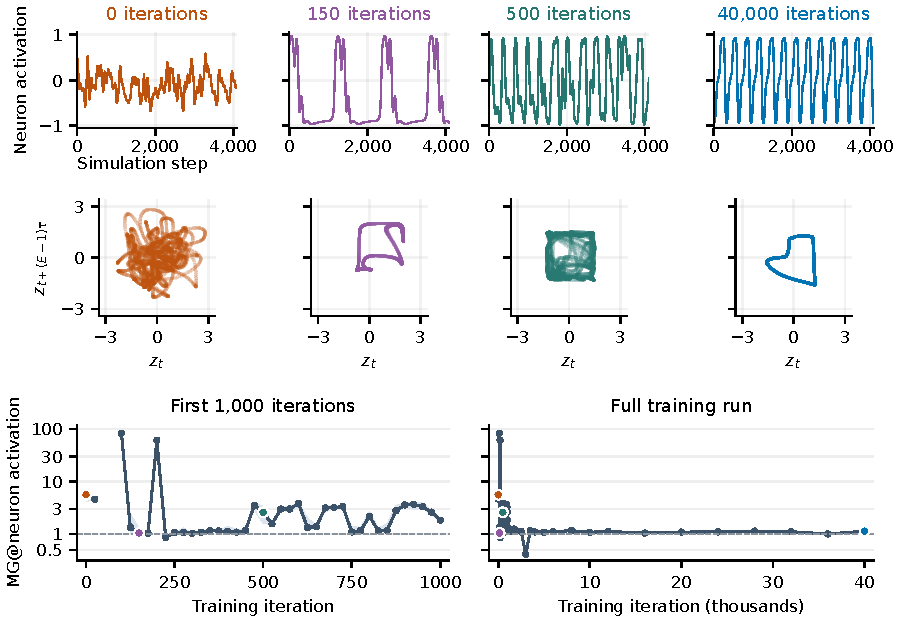
\includegraphics[width=\textwidth]{figures/force_training_transition.pdf}
\caption{Single-neuron activity during FORCE training. The upper panels show separate fixed-weight simulations and \cx{projections of the first window onto the first and last delay coordinates}. The bottom panels show \cx{the median and range across windows within each simulation}. Crosses indicate unavailable estimates, the triangle indicates an off-scale value, and the dashed line marks dimension one.}
\label{fig:force-log-geometry}
\end{figure*}
}
